\documentclass[a4paper,11pt]{article}

\usepackage{graphicx}
\graphicspath{ {./notes/img/} }

\usepackage[activate={true,nocompatibility}]{microtype}
\usepackage[T1]{fontenc}
\usepackage{microtype}
\usepackage[xcharter]{newtx}

\renewcommand{\baselinestretch}{1.05}
\usepackage{graphicx}
\usepackage{inconsolata}
\usepackage[scaled=0.92]{sourcesanspro}
\usepackage{xcolor}
\usepackage[utf8]{inputenc}
\usepackage[english]{babel}
\usepackage[a4paper, left=1.3in, right=1.3in]{geometry}
\usepackage{calc}
\usepackage{graphicx}

\usepackage{titlesec}

\titleformat{\subsubsection}[runin]
  {\normalfont\itshape}
  {\normalfont\bfseries(\thesubsubsection)}
  {1.5\wordsep}
  {}
  [.]

\titlespacing*{\subsubsection}
  {0pt}{6pt}{\wordsep}  % left, before, after spacing

\usepackage{mathpartir}
\usepackage{amsmath}

\usepackage{listings}
\lstdefinestyle{wasm}{
  basicstyle=\ttfamily,
  numberstyle=\footnotesize,
  numbers=left,
  columns=fullflexible,
  numbersep=10pt,
}
\lstset{style=wasm}

\DeclareMathOperator{\reft}{\textsf{ref}}
\DeclareMathOperator{\rect}{\textsf{rec}}
\DeclareMathOperator{\parat}{\textsf{param}}
\DeclareMathOperator{\rest}{\textsf{result}}
\DeclareMathOperator{\strt}{\textsf{struct}}
\DeclareMathOperator{\arrt}{\textsf{array}}
\DeclareMathOperator{\funt}{\textsf{func}}
\DeclareMathOperator{\fldt}{\textsf{field}}
\DeclareMathOperator{\vart}{\textsf{var}}
\DeclareMathOperator{\cstt}{\textsf{const}}
\DeclareMathOperator{\broncast}{\textsf{br\_on\_cast}}
\DeclareMathOperator{\reftest}{\textsf{ref.test}}
\DeclareMathOperator{\localget}{\textsf{local.get}}
\DeclareMathOperator{\refnullt}{\textsf{ref null}}

\usepackage{tikz}
\usepackage{wrapfig}

\usepackage[backend=bibtex, style=alphabetic]{biblatex}
\renewcommand*{\bibfont}{\small}

\title{Towards BBV for Wasm}
\begin{document}
\sloppy
\maketitle
\section{Bouts du rapport de stage sur le BBV}
\subsubsection{Construction of a control-flow graph}
Constructing a CFG from a Wasm program is straightforward except for exceptions
which we don't support yet. One only needs to follow the program's control flow,
while keeping a state of the types on the stack to annotate the basic blocks
with types.

\subsubsection{Reconstruction of Wasm}
As we don't have a general goto instruction, the translation of a CFG to a a
valid Wasm program isn't as easy. To reconstruct structured control flow, we
implement the algorithm described in~\cite{ramsey2022beyond}. This algorithm
relies on the \emph{dominance tree} of the CFG, which we compute using the
algorithm of~\cite{cooper2001simple}. We adaptated Ramsey's algorithm to support
\textsf{br\_on\_cast} as a way to jump out of a block and to use the type
annotations on the CFG to type the Wasm blocks. The latter addition allows
preserving block parameters and output values in the input program.

\subsubsection{Reducibility}
Ramsey's algorithm works on \emph{reducible} CFGs. Intuitively, a CFG is
reducible when each loop has a single entry point. WebAssembly's structured
control flow only produce such CFGs. But the SBBV we work on can modify the CFG
of a program with no guaranty on reducibility, at least in its current
formulation.

\subsubsection{Fixing non-reducibility}
We are considering two different ways to obtain a reducible CFG after this pass.

On the one hand, the GHC compiler, which uses Ramsey's algorithm, makes CFGs
reducible through \emph{node-splitting}. This technique duplicates problematic
nodes such that each copy has a unique incoming arc, until the resulting graph
is reducible. With this method, the reducible graph obtained executes exactly
the same instructions as the original one, at the cost of a size expansion,
which can be exponential~\cite{carter2003folklore}. GHC implements node
splitting~\cite[Appendix~A]{ramsey2022beyond} with a greedy algorithm. A more
elaborate method obtains better results~\cite{janssen1997making}.

On the other hand, non-reducibility appears when SBBV duplicates the head of a
loop and that there are arcs between the different versions of the same loop. We
can then make the graph reducible by creating a new node that serve as a common
head for all the versions of the loop. Instead of jumping to a head, a node
would branch to this new head indicating which version of the loop it targets.
The new head would then branch to one of the previous heads with a
\textsf{br\_table}. This approach solves size explosion problem but adds
execution overhead.

We also plan to test not applying the optimisation to some parts of the graph
where it generates a non-reducible CFG.

\section{Nouvelles idées}
\subsection{Garder un CFG réductible}
On veut garder le CFG réductible en faisant le node \emph{splitting} via BBV\@.
On ajoute aux contextes une pile de têtes de boucle. Quand on veut aller d'une
boucle à une autre (piles de têtes différentes), on crée une copie noeud
d'arrivée qui a le même contexte que le noeud d'arrivée, à part la pile de têtes
où on garde le plus grand préfixe commun (c'est fait dans la fonction
\texttt{reach}) et on applique la même procédure pour les noeuds sortant du
noeud qu'on vient de créer. Par contre si le noeud d'arrivée est une tête de
boucle, le sommet de pile peut-être différent. Ces règles pour la fonction
\texttt{reach} du BBV vont dérouler les boucles jusqu'à atteindre une tête. Ces
ponts entre les boucles peuvent être partagés par plusieurs boucles se rendant à
une même tête.

\begin{center}
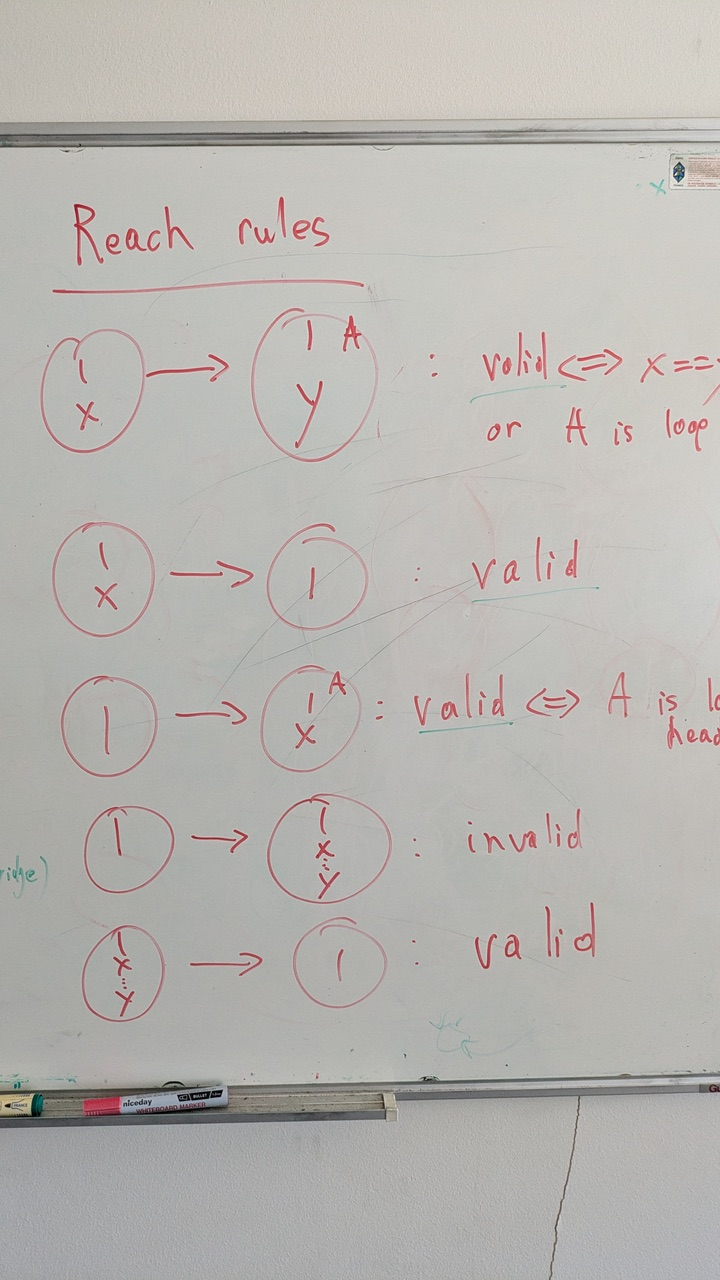
\includegraphics[width=\textwidth]{reach-rules}
\end{center}

Il est possible que des noeuds qui était dans une boucle ne le soit plus après
que BBV (par exemple avec de l'\emph{unrolling}), pour l'instant on envisage de
séparer quand même le noeud en restant conservatif. Une passe supplémentaire à
la fin pourra supprimer les dupliqués inutiles.

\end{document}
